\documentclass[10pt]{beamer}
%\usepackage[latin1]{inputenc}
\usepackage{xmpmulti}
\usetheme{default}
\beamertemplatesolidbackgroundcolor{black}
\setbeamercolor{normal text}{fg=white}
\setbeamercolor{title}{fg=white}
\usecolortheme[named=white]{structure}
\setbeamertemplate{frametitle}[default][center]
\setbeamertemplate{navigation symbols}{}

\title{\texttt{scln}}
\subtitle{An Onion Router for Microcontrollers}
\author{Joseph Colosimo}
\date{December 13, 2011}
\institute{6.858 Final Project}


\begin{document}
\begin{frame}
    \titlepage
\end{frame}

\section{Introduction}

    \begin{frame}{Embedded Devices are Everywhere\ldots}
        \begin{itemize}
            \item<1-> Microcontrollers are in practically everything
            \item<2-> No longer enough that they operate independently
            \item<3-> Lots of research being done in mesh networks
            \item<4-> Networks of devices are the future 
    \end{frame}

    \begin{frame}{\ldots but Security is not}
        \begin{itemize}
            \item<1-> What if you want to tap into a sensor network but you
                don't want data collected about you?
            \item<2-> What if one device wants to send data to another without
                the fear of eavesdropping?
        \end{itemize}
    \end{frame}

\section{Implementation}

    \begin{frame}{\texttt{scln}'s Architecture}
        \begin{center}
            \includegraphics<1>[scale=0.30]{fig/arch.pdf}
        \end{center}
    \end{frame}
    
    \begin{frame}{Testing Framework}
        \begin{center}
            \includegraphics[scale=0.30]{fig/board1.pdf}
        \end{center}
        
        \begin{center}
            \item<2-> Uh\ldots don't we have a problem?
        \end{center}
    \end{frame}

    \begin{frame}{Well, in the Real World}
        \begin{center}
            \includegraphics<1>[scale=0.30]{fig/real1.pdf}
            \includegraphics<2>[scale=0.30]{fig/real2.pdf}
        \end{center}
    \end{frame}
    
    \begin{frame}{Demo}
        \begin{center}
            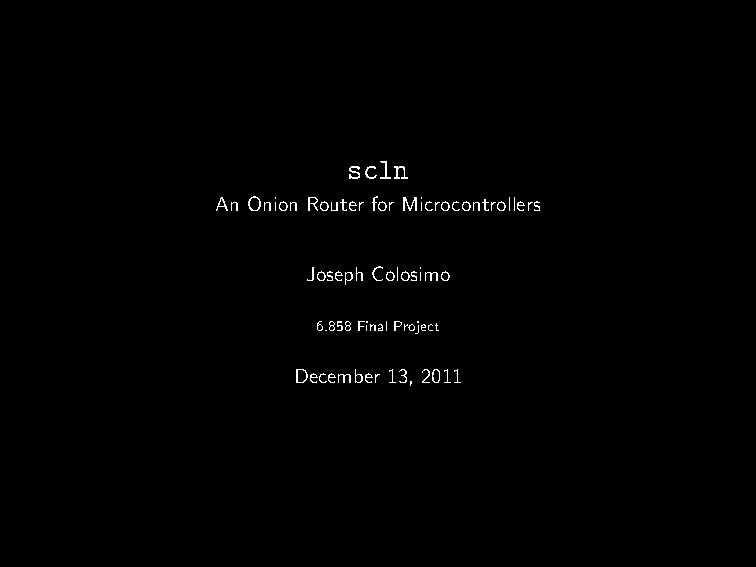
\includegraphics[scale=0.30]{fig/demo.pdf}
        \end{center}
    \end{frame}
        
\end{document}
